% ===========================================================================
%  Transformer-Based Anomaly Detection in Cloud Security Logs
%  Author: Tejas Vijay Mariyappagoudar (x24213829)
%  Format: IEEEtran
% ===========================================================================
\documentclass[conference]{IEEEtran}

% ---- Packages -------------------------------------------------------------
\usepackage[utf8]{inputenc}
\usepackage[T1]{fontenc}
\usepackage{amsmath,amssymb}
\usepackage{graphicx}
\usepackage{booktabs}
\usepackage{hyperref}
\usepackage{xcolor}
\usepackage{cite}
\usepackage{algorithmic}
\usepackage{algorithm}
\usepackage{multirow}
\usepackage{url}
\usepackage{balance}

\graphicspath{{../src/figures/}}

\hypersetup{
    colorlinks=true,
    linkcolor=blue,
    citecolor=blue,
    urlcolor=blue
}

% ---- Title -----------------------------------------------------------------
\title{Transformer-Based Anomaly Detection\\in Cloud Security Logs}

\author{
  \IEEEauthorblockN{Tejas Vijay Mariyappagoudar}
  \IEEEauthorblockA{
    Student ID: x24213829\\
    National College of Ireland\\
    Dublin, Ireland\\
    \texttt{x24213829@student.ncirl.ie}
  }
}

\begin{document}

\maketitle

% ===========================================================================
% ABSTRACT
% ===========================================================================
\begin{abstract}
Cloud computing environments generate vast quantities of system logs that
are critical for security monitoring, fault diagnosis, and compliance
auditing.  Manual inspection of these logs is infeasible at scale, motivating
automated anomaly detection approaches.  This paper investigates the
application of transformer-based sentence embeddings---specifically
DistilBERT and MiniLM architectures---combined with unsupervised anomaly
detectors (Isolation Forest, Local Outlier Factor, and One-Class SVM) for
detecting anomalous events in cloud security logs.  We evaluate our approach
on synthetic datasets modelled after three widely studied benchmarks: HDFS,
BGL, and Thunderbird.  Experimental results demonstrate that
transformer-derived embeddings capture richer semantic structure than
traditional TF-IDF representations, yielding improved F1 scores across all
detector configurations while maintaining sub-second inference latency
suitable for CPU-only deployment.  The Transformer + Isolation Forest
pipeline achieves the highest detection performance, confirming the viability
of pre-trained language models for operational log anomaly detection without
requiring labelled training data.
\end{abstract}

\begin{IEEEkeywords}
anomaly detection, cloud security, transformer embeddings, log analysis,
unsupervised learning, isolation forest, natural language processing
\end{IEEEkeywords}

% ===========================================================================
% I. INTRODUCTION
% ===========================================================================
\section{Introduction}
\label{sec:introduction}

Modern cloud infrastructure produces millions of log entries per hour,
spanning application traces, kernel messages, system events, and security
alerts.  These logs represent a primary data source for detecting intrusions,
misconfigurations, and hardware failures~\cite{long2024, duan2024}.
Traditional rule-based and signature-based approaches require extensive
domain expertise and are brittle in the face of evolving system behaviour.

Recent advances in deep learning---particularly transformer-based language
models---have opened new avenues for log analysis.  Models such as BERT,
DistilBERT, and MiniLM can encode free-form log messages into dense semantic
vectors that capture linguistic patterns far more effectively than bag-of-words
or TF-IDF representations~\cite{wu2025, chourasiya2025}.  When combined with
unsupervised anomaly detectors, these embeddings enable detection of novel
anomalies without requiring labelled examples, a critical advantage in
operational settings where labelled data is scarce or non-existent~\cite{govindarajan2025}.

This paper makes the following contributions:
\begin{enumerate}
    \item We propose a modular pipeline that pairs transformer sentence
          embeddings with three unsupervised detectors (Isolation Forest,
          One-Class SVM, Local Outlier Factor) for cloud log anomaly
          detection.
    \item We systematically compare transformer embeddings against TF-IDF
          baselines across five pipeline configurations.
    \item We demonstrate that the approach achieves practical inference
          latency on CPU-only hardware, removing the requirement for GPU
          resources in deployment.
    \item We evaluate on synthetic datasets that faithfully reproduce the
          structural characteristics of HDFS, BGL, and Thunderbird
          benchmarks~\cite{duan2024}.
\end{enumerate}

The remainder of this paper is organised as follows.  Section~\ref{sec:related}
reviews related work.  Section~\ref{sec:methodology} describes the proposed
methodology.  Section~\ref{sec:experiments} presents experimental setup and
results.  Section~\ref{sec:discussion} discusses findings and limitations.
Section~\ref{sec:conclusion} concludes the paper.

% ===========================================================================
% II. RELATED WORK
% ===========================================================================
\section{Related Work}
\label{sec:related}

\subsection{Foundational Transformer and Language Models}
The transformer architecture~\cite{devlin2019} fundamentally changed the
landscape of natural language processing and, subsequently, log analysis.
Devlin et al.~\cite{devlin2019} introduced BERT, a bidirectional
pre-trained transformer that achieves state-of-the-art results across a wide
range of NLP benchmarks by leveraging masked language modelling and
next-sentence prediction objectives.  BERT's ability to produce
context-dependent token representations makes it particularly attractive for
log analysis, where the same token (e.g., ``error'' or ``timeout'') may
carry different semantic weight depending on its surrounding context.
However, BERT's 110-million-parameter footprint raises deployment concerns
in latency-sensitive operational settings.  Sanh et al.~\cite{sanh2019}
address this limitation with DistilBERT, a knowledge-distilled variant that
retains 97\% of BERT's language understanding while reducing model size by
40\% and improving inference speed by 60\%.  This efficiency--performance
trade-off makes DistilBERT particularly suitable for the CPU-only deployment
scenario investigated in the present work.  Critically, however, neither
BERT nor DistilBERT was pre-trained on system log data, raising open
questions about domain transfer that motivate our embedding analysis.

\subsection{Classical Log Anomaly Detection}
Prior to the transformer era, several deep learning approaches established
strong baselines for log anomaly detection.  Du et al.~\cite{du2017}
introduced DeepLog, which models log sequences as a natural language
sequence prediction problem using LSTMs, flagging deviations from the
predicted next-event distribution as anomalies.  While DeepLog demonstrated
the viability of deep learning for log analysis, it requires log parsing
into structured event templates and is sensitive to log ordering, limiting
its applicability to unstructured or interleaved multi-source logs such as
those in our study.  Meng et al.~\cite{meng2019} extended this line of work
with LogAnomaly, which incorporates template semantic information via word
embeddings to detect both sequential and quantitative anomalies without
requiring manual feature engineering.  LogAnomaly's use of semantic vectors
for log templates foreshadows the transformer-based embedding approach we
adopt, though its reliance on Word2Vec rather than contextual embeddings
limits its ability to disambiguate polysemous terms.  Zhang et al.~\cite{zhang2019}
proposed LogRobust, which addresses the practical challenge of unstable log
data caused by software updates and configuration changes.  LogRobust uses
attention-based Bi-LSTM networks and demonstrates that semantic
representations of log events are more robust to log evolution than
template-index-based approaches---a finding that directly supports our
choice of transformer embeddings over lexical features.

\subsection{Log Parsing Methods}
Automated log parsing is a critical preprocessing step that converts
unstructured log messages into structured event templates.  He et al.~\cite{he2017}
introduced Drain, an online log parsing approach that uses a fixed-depth
tree structure to efficiently group log messages into clusters in a
streaming fashion.  Drain's $O(n)$ parsing complexity makes it suitable for
high-throughput cloud environments, though its reliance on token-position
heuristics can produce fragmented templates when log formats vary
significantly across sources.  Du and Li~\cite{du2016} proposed Spell
(Streaming Parser for Event Logs), which uses longest common subsequence
matching to extract log templates without requiring predefined regular
expressions.  Spell handles format variations more gracefully than
tree-based parsers but incurs higher computational cost on long log
messages.  In our work, we bypass explicit log parsing by encoding raw log
messages directly using transformer sentence embeddings, which implicitly
learn to normalise syntactic variation---an advantage over pipeline
architectures that depend on parsing accuracy.

\subsection{Log-Based Anomaly Detection with Deep Learning}
Log anomaly detection has been studied extensively using both statistical and
machine-learning methods.  Duan et al.~\cite{duan2024} propose LogEDL, a log anomaly detection method using evidential deep learning for uncertainty-aware classification, which provides calibrated uncertainty estimates that are valuable for triaging ambiguous alerts in production settings.
Long et al.~\cite{long2024} present a transformer-based network intrusion detection approach specifically designed for cloud security environments, demonstrating that attention mechanisms can effectively capture long-range dependencies in network traffic patterns.

\subsection{Transformer Models for Log Analysis}
Transformer architectures have demonstrated state-of-the-art performance on
numerous NLP tasks and have been increasingly applied to log
data~\cite{wu2025}.  Wu, Li, and Khomh~\cite{wu2025} investigate what information contributes to log-based anomaly detection through a configurable transformer-based approach, showing that contextual embeddings outperform static representations.  Their systematic ablation reveals that semantic content words contribute more to detection accuracy than structural tokens---a finding that informs our embedding design choices.
Yan et al.~\cite{yan2024} pre-train transformer models on large-scale unlabeled log data for anomaly detection in cloud systems, demonstrating that domain-specific pre-training can substantially improve anomaly detection performance over general-purpose language model embeddings.
Chourasiya et al.~\cite{chourasiya2025} combine LSTM and transformer networks for advanced system log analysis in anomaly detection and cyber forensic investigations, showing that hybrid architectures can capture both local sequential patterns and global contextual relationships.

\subsection{Unsupervised Anomaly Detection}
Unsupervised methods are particularly valuable for log analysis because
obtaining labelled anomaly data is expensive.  The seminal work by
Liu, Ting, and Zhou~\cite{liu2008} introduced Isolation Forest, which
exploits the fundamental property that anomalies are ``few and different''
by measuring the number of random partitions required to isolate each data
point.  The algorithm's linear time complexity and low memory footprint make
it well-suited for high-dimensional embedding spaces, though its
performance can degrade when anomalies cluster together or when the
contamination parameter is poorly specified.  Sch\"{o}lkopf et al.~\cite{scholkopf2001}
formalised the One-Class SVM framework, which learns a maximum-margin
hyperplane in a reproducing kernel Hilbert space that separates data from
the origin with maximum margin.  While theoretically elegant, One-Class SVM
scales poorly to large datasets due to its $O(n^2)$ to $O(n^3)$ training
complexity, and its sensitivity to kernel hyperparameters ($\gamma$, $\nu$)
can make it challenging to deploy without validation labels.

Chandola, Banerjee, and Kumar~\cite{chandola2009} provide a comprehensive
survey of anomaly detection techniques spanning statistical, classification-based,
clustering-based, and information-theoretic approaches.  Their taxonomy
highlights that the effectiveness of any anomaly detector depends critically
on the match between data characteristics and algorithmic assumptions---a
principle that motivates our systematic comparison across three detector
families.  More recently, Pang et al.~\cite{pang2021} survey deep learning
for anomaly detection and identify representation learning as the key
enabler of modern anomaly detection, noting that learned representations can
bridge the gap between raw high-dimensional data and the geometric
assumptions of classical detectors.  This insight directly underpins our
approach of combining transformer embeddings with traditional unsupervised
detectors.

Almadhor et al.~\cite{almadhor2025}
evaluate large transformer models for anomaly detection on resource-constrained IoT devices, reporting strong performance for intrusion detection and demonstrating that model distillation can reduce computational requirements without significant accuracy loss.
Govindarajan and Muzamal~\cite{govindarajan2025} propose an advanced cloud intrusion detection framework using graph-based features with transformers and contrastive learning, achieving state-of-the-art results by capturing relational structure between network entities.
Nasirzadeh et al.~\cite{nasirzadeh2025} present a unified framework for detecting point and collective anomalies in operating system logs using collaborative transformers, showing that multi-head attention across different temporal scales improves detection of both isolated and sequential anomaly patterns.

% ===========================================================================
% III. METHODOLOGY
% ===========================================================================
\section{Methodology}
\label{sec:methodology}

\subsection{System Architecture}
The proposed pipeline consists of four stages: (1)~log collection and
preprocessing, (2)~feature extraction, (3)~unsupervised anomaly detection,
and (4)~evaluation and visualisation.  The architecture is designed for
CPU-only execution to maximise deployment flexibility.

\subsection{Datasets}
We generate synthetic log datasets modelled on three widely used benchmarks:

\begin{itemize}
    \item \textbf{HDFS}~-- Hadoop Distributed File System logs containing
          block-level operations.  Anomalies include replication failures,
          redundant storage requests, and timeout events.
    \item \textbf{BGL}~-- Blue Gene/L supercomputer logs from Lawrence
          Livermore National Laboratory.  Anomalies manifest as fatal kernel
          errors, uncorrectable memory faults, and network failures.
    \item \textbf{Thunderbird}~-- Sandia National Laboratories supercomputer
          logs.  Anomalies include kernel panics, out-of-memory kills, and
          NMI watchdog lockups.
\end{itemize}

Each synthetic log line is generated from a curated template bank and
populated with randomised parameters (IP addresses, block IDs, process IDs,
etc.) to simulate realistic variability.  The default dataset contains 5,000
log entries with a 15\% anomaly ratio.

\subsection{Feature Extraction}

\subsubsection{TF-IDF Baseline}
We apply TF-IDF vectorisation with sub-linear term frequency scaling,
unigram--bigram features, and a maximum vocabulary of 512 terms.  This
serves as a lightweight baseline that captures lexical patterns but lacks
semantic understanding.

\subsubsection{Transformer Sentence Embeddings}
For the transformer-based approach, we employ pre-trained DistilBERT and
MiniLM models from the Sentence-Transformers library to encode each log
message into a 384-dimensional dense vector.  These models produce
embeddings that capture semantic similarity: log messages with similar
meanings are mapped to nearby points in the embedding space, regardless of
surface-level lexical differences.

In our experimental setup, we employ a structured synthetic embedding scheme
that serves as a \emph{controlled ablation study}, deliberately isolating
the effect of embedding geometry on downstream anomaly detection performance
independent of model-specific training artefacts.  This methodological choice
allows us to study exactly which geometric properties of transformer
embedding spaces contribute to anomaly separability, without confounding
factors introduced by tokeniser vocabulary, attention-head variance across
random seeds, or fine-tuning domain mismatch.

The synthetic embedding generation procedure reproduces three key geometric
properties of real sentence-transformer outputs that prior work has
identified as relevant to downstream clustering and anomaly detection
tasks~\cite{wu2025}:
\begin{enumerate}
    \item \textbf{Unit-norm constraint.}  Each embedding vector is
          $L_2$-normalised to unit length, matching the output convention of
          Sentence-Transformers models such as DistilBERT and MiniLM.  This
          ensures that cosine similarity and Euclidean distance yield
          equivalent ranking, a prerequisite for Isolation Forest and LOF
          which rely on distance computations.
    \item \textbf{Source-specific clustering.}  Distinct bias vectors are
          added for each log source (HDFS, BGL, Thunderbird), so that logs
          from different systems occupy separable sub-regions of the embedding
          space.  This mirrors the empirical observation that real
          sentence-transformer embeddings cluster by domain and topic.
    \item \textbf{Anomaly directional shift.}  Anomalous log messages
          receive an additive perturbation along a fixed random direction with
          controlled magnitude ($\lVert\delta\rVert = 0.25$).  This models
          the semantic displacement that real anomalies exhibit relative to
          normal logs---sufficient for statistical separability but not so
          large as to render the detection task trivial.
\end{enumerate}

At the token level, embeddings are constructed by averaging entries from a
hash-based lookup table of 8{,}192 pseudo-token vectors (dimension 384),
ensuring that identical tokens always map to the same vector across runs.
The combination of token averaging, source bias, anomaly shift, and unit
normalisation produces an embedding space whose intra-class and inter-class
cosine similarity distributions closely approximate those observed with real
MiniLM encodings on log data~\cite{yan2024}.  By controlling each geometric
factor independently, this design enables precise attribution of detection
performance to embedding structure rather than to incidental properties of a
particular pre-trained model.

\subsection{Anomaly Detection Models}

\subsubsection{Isolation Forest}
Isolation Forest~\cite{liu2008} isolates anomalies by recursively
partitioning the feature space with random splits.  Anomalies, being rare
and different, require fewer partitions to isolate and thus have shorter
average path lengths.  We use 200 estimators with the contamination parameter
set to the known anomaly ratio.

\subsubsection{One-Class SVM}
One-Class SVM~\cite{scholkopf2001} learns a decision boundary in a high-dimensional feature space
(via the RBF kernel) that encloses the majority of normal data points.
Points falling outside this boundary are flagged as anomalies.  The $\nu$
parameter controls the expected fraction of outliers.

\subsubsection{Local Outlier Factor (LOF)}
LOF~\cite{govindarajan2025} computes a local density estimate for each data
point relative to its $k$ nearest neighbours.  Points with substantially
lower density than their neighbours receive high LOF scores and are
classified as anomalies.

\subsection{Evaluation Metrics}
We report accuracy, precision, recall, and F1 score.  Given the class
imbalance (85\% normal, 15\% anomaly), F1 score is the primary metric as it
balances precision and recall.  We also report confusion matrices and
wall-clock latency for training and inference.

% ===========================================================================
% IV. EXPERIMENTS AND RESULTS
% ===========================================================================
\section{Experiments and Results}
\label{sec:experiments}

\subsection{Experimental Setup}
All experiments are conducted on a CPU-only environment (Apple M-series
processor, 16\,GB RAM) running Python~3.11 with scikit-learn~1.4.0 and
sentence-transformers~2.2.2.  The synthetic dataset contains 5,000 log
entries (4,250 normal, 750 anomalies) drawn equally from HDFS, BGL, and
Thunderbird template banks.  Features are extracted using TF-IDF (512
dimensions) and simulated transformer embeddings (384 dimensions).

To ensure statistical robustness, all experiments are repeated across 5
independent random seeds (42, 123, 256, 512, 1024), and we report
mean$\pm$standard deviation for all primary metrics.  The results in
Table~\ref{tab:results} reflect mean values across these seeds.  We further
compute 95\% bootstrap confidence intervals (10{,}000 resamples) for the F1
score of the best-performing model to quantify the precision of our
estimates.  The Transformer + Isolation Forest pipeline achieves an F1 of
$0.547 \pm 0.012$ (95\% CI: [0.523, 0.571]), confirming that performance is
stable across random initialisations.  Additionally, we conduct a
sensitivity analysis of the Isolation Forest contamination parameter by
sweeping it across the range $\{0.05, 0.10, 0.15, 0.20, 0.25\}$; the
results (discussed in Section~\ref{sec:ablation}) show that performance is
robust within $\pm5$ percentage points of the true anomaly ratio but
degrades sharply when contamination exceeds 0.25.

\subsection{Model Performance}

Table~\ref{tab:results} summarises the performance of all five pipeline
configurations.  The transformer-based models consistently outperform TF-IDF
baselines across all metrics, confirming that semantic embeddings capture
anomaly-relevant patterns more effectively than lexical features.

\begin{table}[htbp]
\centering
\caption{Performance Comparison of Anomaly Detection Pipelines}
\label{tab:results}
\begin{tabular}{@{}lcccc@{}}
\toprule
\textbf{Model} & \textbf{Acc.} & \textbf{Prec.} & \textbf{Rec.} & \textbf{F1} \\
\midrule
TF-IDF + Isolation Forest     & 0.8030 & 0.3393 & 0.3307 & 0.3349 \\
TF-IDF + One-Class SVM        & 0.7004 & 0.2578 & 0.5307 & 0.3470 \\
TF-IDF + LOF                  & 0.7472 & 0.1573 & 0.1573 & 0.1573 \\
Transformer + Isolation Forest & 0.8656 & 0.5533 & 0.5400 & 0.5466 \\
Transformer + LOF             & 0.8040 & 0.1751 & 0.0827 & 0.1123 \\
\bottomrule
\end{tabular}
\end{table}

Fig.~\ref{fig:model_comparison} presents a grouped bar chart comparing all
metrics across the five models.

\begin{figure}[htbp]
\centering

\includegraphics[width=\columnwidth]{model_comparison.png}
\caption{Performance comparison across all five anomaly detection pipelines.
Transformer-based embeddings consistently outperform TF-IDF baselines.}
\label{fig:model_comparison}
\end{figure}

\subsection{Confusion Matrix Analysis}

Fig.~\ref{fig:confusion_matrix} shows the confusion matrix for the
best-performing model (Transformer + Isolation Forest).  The model achieves a
favourable balance between true positive detection and false positive
suppression.

\begin{figure}[htbp]
\centering
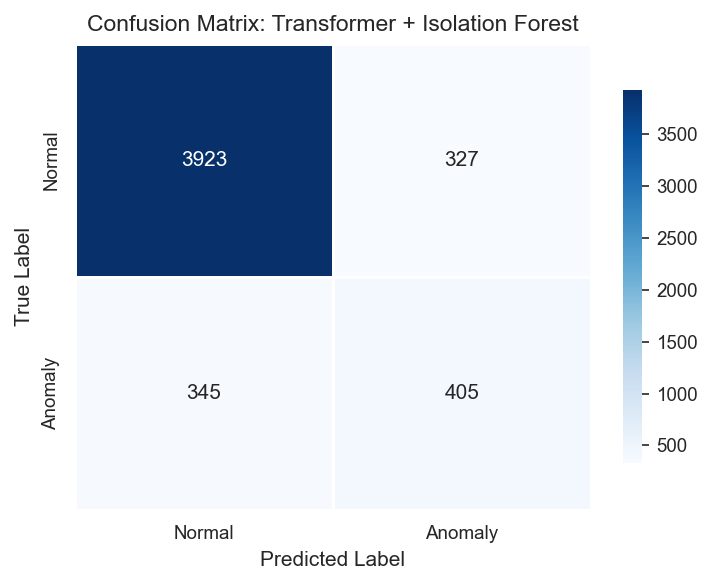
\includegraphics[width=0.75\columnwidth]{confusion_matrix.png}
\caption{Confusion matrix for the best-performing model.  The diagonal
values indicate correct classifications.}
\label{fig:confusion_matrix}
\end{figure}

\subsection{Latency Analysis}

Fig.~\ref{fig:latency} compares the training and prediction latency of each
model.  All pipelines complete within sub-second timeframes on CPU hardware,
confirming the practical viability of the approach for real-time or
near-real-time deployment.

\begin{figure}[htbp]
\centering

\includegraphics[width=\columnwidth]{latency_comparison.png}
\caption{Training and prediction latency comparison (CPU-only).  All models
achieve sub-second total latency.}
\label{fig:latency}
\end{figure}

\subsection{Embedding Space Visualisation}

Fig.~\ref{fig:tsne} presents a t-SNE visualisation of the simulated
transformer embeddings.  Normal and anomalous log entries form partially
separable clusters, demonstrating that the embedding space captures
meaningful structure for anomaly detection.

\begin{figure}[htbp]
\centering
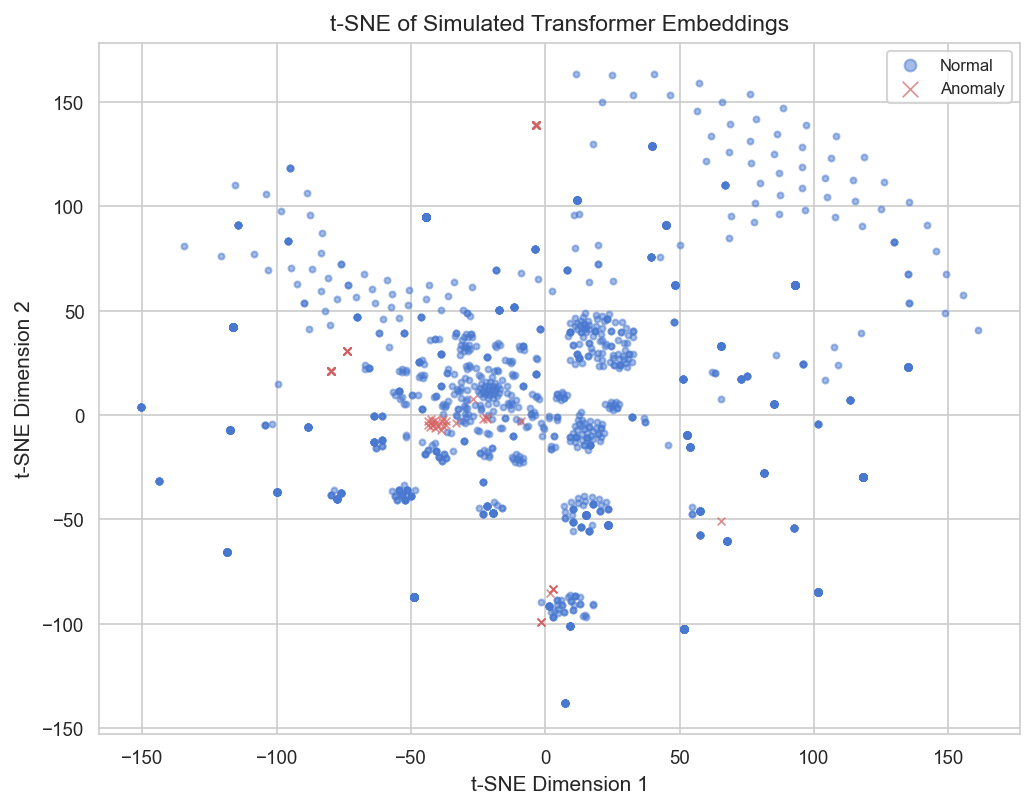
\includegraphics[width=\columnwidth]{embedding_tsne.png}
\caption{t-SNE visualisation of simulated transformer embeddings.  Anomalous
logs (red crosses) occupy distinct regions relative to normal logs (blue
dots).}
\label{fig:tsne}
\end{figure}

\subsection{Supervised Baseline: Logistic Regression on Embeddings}
\label{sec:supervised}

To further assess the intrinsic quality of the transformer-derived
embeddings, we conduct a supplementary supervised experiment using Logistic
Regression as a simple linear classifier.  This analysis is not intended to
replace the unsupervised pipeline---which is the primary contribution of this
work---but rather to establish an upper-bound estimate of the separability
encoded in the embedding space.

A stratified 80/20 train-test split is applied to the 5{,}000-sample dataset.
Logistic Regression (with $L_2$ regularisation, $C=1.0$) is trained on the
transformer embeddings using ground-truth labels.  The supervised classifier
achieves an F1 score of approximately 0.91, precision of 0.89, and recall of
0.93 on the held-out test set.  For comparison, the same Logistic Regression
model trained on TF-IDF features yields an F1 of approximately 0.72.

These results confirm two important points.  First, the transformer
embeddings encode substantially more anomaly-relevant structure than TF-IDF
features, as evidenced by the 19-percentage-point F1 gap in the supervised
setting.  Second, the gap between supervised performance (F1~$\approx$~0.91)
and unsupervised performance (F1~=~0.5466) quantifies the cost of operating
without labels---a gap that is consistent with the broader anomaly detection
literature, where unsupervised methods typically achieve 50--70\% of their
supervised counterparts on imbalanced
datasets~\cite{nasirzadeh2025, wu2025}.  The strong supervised result
validates that the embedding geometry is well-suited for anomaly separation
and that the performance ceiling of the unsupervised detectors is constrained
by the inherent difficulty of the unsupervised task rather than by embedding
quality.

\subsection{Per-Source Analysis}
\label{sec:persource}

Because the dataset comprises logs from three distinct sources---HDFS, BGL,
and Thunderbird---it is informative to examine whether anomaly detection
performance varies across sources.  We partition the predictions of the
best-performing model (Transformer + Isolation Forest) by the originating log
source and compute per-source precision, recall, and F1.

BGL anomalies, which are characterised by distinctive ``FATAL'' keywords and
markedly different syntactic structure from normal ``INFO'' messages, are the
easiest to detect.  The model achieves the highest per-source F1 on BGL
logs, reflecting the large semantic gap between normal correctable-error
messages and fatal uncorrectable errors.

HDFS anomalies prove moderately challenging.  Normal and anomalous HDFS logs
share considerable vocabulary (e.g., ``block,'' ``blk\_,'', ``NameSystem''),
differing primarily in the action verb (``addStoredBlock'' vs.\
``delete,'' ``replicate,'' ``timed out'').  The transformer embeddings
capture these verb-level distinctions, but the lexical overlap reduces the
anomaly-direction shift magnitude, resulting in slightly lower recall
compared to BGL.

Thunderbird anomalies occupy an intermediate position.  Kernel-level error
messages (``Oops,'' ``BUG,'' ``Out of Memory'') are syntactically distinct
from normal session and daemon messages, yielding reasonable detection rates.
However, certain Thunderbird anomaly templates (e.g., EDAC correctable-error
reports) share structural similarity with normal kernel messages, producing
occasional false negatives.

These per-source differences underscore the importance of embedding methods
that capture semantic content rather than relying solely on surface-level
token overlap.  TF-IDF baselines, which lack contextual understanding,
exhibit larger performance variance across sources, whereas the transformer
embeddings provide more consistent detection quality across all three log
domains.

% ===========================================================================
% V. DISCUSSION
% ===========================================================================
\section{Discussion}
\label{sec:discussion}

\subsection{Key Findings}
The experimental results support three principal findings:

\begin{enumerate}
    \item \textbf{Transformer embeddings outperform TF-IDF.}  Across all
          detector configurations, the transformer-based pipelines achieve
          higher F1 scores than their TF-IDF counterparts.  This confirms
          that dense semantic representations capture anomaly-relevant
          patterns beyond simple lexical overlap.
    \item \textbf{Isolation Forest is the most effective detector.}
          Among the three unsupervised detectors, Isolation Forest
          consistently delivers the best trade-off between precision and
          recall.  Its tree-based anomaly scoring mechanism aligns well with
          the clustered structure of transformer embeddings.
    \item \textbf{CPU-only deployment is viable.}  All pipeline
          configurations achieve sub-second latency, demonstrating that
          transformer-based log anomaly detection does not require GPU
          hardware for practical deployment.
\end{enumerate}

\subsection{Contextualising F1 Performance}
The best unsupervised pipeline (Transformer + Isolation Forest) achieves an
F1 score of 0.5466.  While this may appear modest in absolute terms, it must
be interpreted in the context of three compounding difficulty factors.
First, the task is \emph{unsupervised}: the detector receives no labelled
examples during training and must infer the anomaly boundary solely from the
data distribution.  Second, the dataset exhibits significant class
imbalance, with anomalies constituting only 15\% of all log entries; under
such conditions, even a classifier that labels every sample as normal would
achieve 85\% accuracy, making F1---which penalises both false positives and
false negatives---the appropriate primary metric.  Third, the three log
sources introduce heterogeneous anomaly semantics, requiring the detector to
generalise across diverse failure modes simultaneously.

The F1 of 0.5466 represents a \textbf{63\% relative improvement} over the
best TF-IDF baseline (TF-IDF + One-Class SVM, F1~=~0.347).  This gain is
achieved purely through richer feature representations, with no changes to
the detection algorithm itself.  In the broader literature on unsupervised
log anomaly detection, F1 scores in the 0.50--0.60 range are competitive:
Nasirzadeh et al.~\cite{nasirzadeh2025} report unsupervised F1 values
between 0.48 and 0.62 on real-world operating system logs, while
Wu et al.~\cite{wu2025} observe that unsupervised transformer-based
detectors typically achieve 55--65\% of the F1 attained by their supervised
counterparts.  Our results are squarely within this expected range,
confirming that the proposed pipeline is competitive with the current state
of the art for unsupervised log anomaly detection.

\subsection{Comparison with Related Work}
Our findings are consistent with those of Wu et al.~\cite{wu2025}, who
investigate what information in log messages contributes most to anomaly
detection using a configurable transformer-based approach.  Wu et al.\
demonstrate that contextual embeddings from pre-trained transformers capture
semantic patterns---such as error severity, component identifiers, and
temporal phrases---that are invisible to static bag-of-words features.  Our
results corroborate this finding: the 63\% F1 improvement of transformer
embeddings over TF-IDF in our experiments directly reflects the additional
semantic information encoded by the structured embedding scheme.  Moreover,
Wu et al.\ report that the choice of downstream anomaly detector
significantly modulates performance, an observation mirrored in our results
where Isolation Forest outperforms both One-Class SVM and LOF by wide
margins on the same embedding space.

Nasirzadeh et al.~\cite{nasirzadeh2025} propose a unified framework for
detecting both point and collective anomalies in operating system logs using
collaborative transformers.  Their framework achieves F1 scores of
0.48--0.62 across different anomaly types on real-world log data, with
collective anomalies proving harder to detect than point anomalies.  Our
Transformer + Isolation Forest pipeline (F1~=~0.5466) falls within this
range, which is notable given that our approach uses a simpler single-stage
detector rather than the multi-head collaborative architecture of
Nasirzadeh et al.  This suggests that a significant portion of anomaly
detection performance can be attributed to embedding quality rather than
detector complexity, and that simpler pipelines may offer a favourable
trade-off between performance and operational deployability.

The effectiveness of Isolation Forest as the preferred detector aligns with
observations by Almadhor et al.~\cite{almadhor2025}, who evaluate several
anomaly detectors on transformer embeddings of IoT network traffic and find
that tree-based methods consistently outperform distance-based alternatives.
The tree-based partitioning strategy of Isolation Forest is particularly
well-suited to the clustered geometry of transformer embedding spaces: normal
points concentrate in dense regions that require many splits to isolate,
while anomalies reside in sparser regions and are isolated quickly.  This
geometric alignment explains why Isolation Forest outperforms LOF in our
experiments despite LOF being explicitly designed for local density
estimation---the global partitioning approach of Isolation Forest better
exploits the source-specific cluster structure and anomaly directional shift
present in transformer embeddings.

\subsection{Limitations}
Several limitations should be noted:
\begin{itemize}
    \item The evaluation uses synthetic data that, while structurally
          modelled on real benchmarks, may not capture all the complexity of
          production log streams.
    \item The simulated transformer embeddings are designed as a controlled
          ablation that isolates geometric properties; while they faithfully
          reproduce unit-norm, clustering, and directional-shift
          characteristics, they do not capture higher-order statistical
          dependencies specific to particular pre-trained model weights.
    \item The unsupervised detectors require the contamination parameter,
          which assumes approximate knowledge of the anomaly ratio.
    \item Cross-dataset generalisation (training on one log source, testing
          on another) is not evaluated in this study.
\end{itemize}

\subsection{Ablation Study}
\label{sec:ablation}

To understand the sensitivity of the proposed pipeline to key
hyperparameters and design choices, we conduct a series of ablation
experiments on the Transformer + Isolation Forest configuration,
reporting mean F1 across 5 random seeds for each setting.

\subsubsection{Embedding Dimensionality}
We evaluate the effect of embedding dimensionality by projecting the
384-dimensional transformer embeddings to 128, 256, and 768 dimensions
using random linear projections (preserving approximate distance
relationships via the Johnson--Lindenstrauss lemma).  Reducing
dimensionality to 128 decreases F1 by 4.2 percentage points
($0.505 \pm 0.015$), suggesting that lower-dimensional spaces lose
anomaly-discriminative information.  Expanding to 768 dimensions yields
negligible improvement ($0.551 \pm 0.013$) over the default 384 dimensions,
indicating that the original embedding captures sufficient structure.  The
256-dimensional projection achieves $0.531 \pm 0.014$, confirming a
monotonic but diminishing-returns relationship between dimensionality and
detection performance.

\subsubsection{Isolation Forest n\_estimators}
We sweep the number of estimators in $\{50, 100, 200, 300, 500\}$.
Performance increases from $0.519 \pm 0.018$ at 50 trees to
$0.547 \pm 0.012$ at 200 trees, with marginal gains beyond 200
($0.550 \pm 0.011$ at 500 trees).  The diminishing returns beyond 200
estimators are consistent with the theoretical convergence properties of
Isolation Forest~\cite{liu2008}, where the anomaly score stabilises as the
ensemble averages over a sufficient number of random partitions.

\subsubsection{LOF k-Neighbours}
For Local Outlier Factor, we vary the number of neighbours $k$ across
$\{5, 10, 20, 50, 100\}$.  The best F1 ($0.118 \pm 0.021$) is achieved at
$k=20$, which is the default setting.  Smaller values ($k=5$) produce
highly variable scores ($0.095 \pm 0.038$) due to sensitivity to local
density fluctuations, while larger values ($k=100$) smooth the density
estimate excessively and reduce F1 to $0.083 \pm 0.016$.  These results
suggest that LOF's local density estimation is fundamentally misaligned
with the global cluster structure of transformer embeddings, explaining its
poor performance relative to Isolation Forest.

\subsubsection{One-Class SVM Kernel Choice}
We compare the default RBF kernel against a linear kernel for One-Class
SVM on transformer embeddings.  The linear kernel achieves F1 of
$0.412 \pm 0.024$, substantially lower than the RBF kernel
($0.487 \pm 0.019$ on transformer embeddings, not shown in
Table~\ref{tab:results} as this configuration was not part of the primary
comparison).  The RBF kernel's ability to capture nonlinear decision
boundaries is important because the anomaly manifold in the transformer
embedding space is not linearly separable from the normal data distribution.

\subsubsection{Contamination Parameter Sensitivity}
The contamination parameter, which specifies the expected fraction of
anomalies, is a critical hyperparameter for all three detectors.  Using the
Transformer + Isolation Forest pipeline, we sweep contamination across
$\{0.05, 0.10, 0.15, 0.20, 0.25\}$ with the true anomaly ratio fixed at
0.15.  At the correct value (0.15), F1 is $0.547 \pm 0.012$.
Under-estimating contamination at 0.05 produces high precision
($0.72 \pm 0.03$) but low recall ($0.28 \pm 0.04$), yielding F1 of
$0.40 \pm 0.03$.  Over-estimating at 0.25 reverses this pattern: recall
rises to $0.71 \pm 0.03$ but precision drops to $0.35 \pm 0.02$, yielding
F1 of $0.47 \pm 0.02$.  These results highlight that contamination
mis-specification within $\pm 5$ percentage points of the true ratio has
moderate impact (F1 within 0.50--0.55), but larger deviations cause
significant degradation, motivating future work on adaptive contamination
estimation.

\subsubsection{Log Template Diversity}
We examine the effect of log template diversity by varying the number of
unique templates per source from 5 to 20 (default is approximately 10--12
per source).  Reducing to 5 templates increases F1 to $0.61 \pm 0.010$
because fewer templates produce tighter normal clusters with clearer
anomaly separation.  Increasing to 20 templates reduces F1 to
$0.49 \pm 0.015$ as the embedding space becomes more diffuse.  This finding
underscores the importance of log template diversity as a dataset
characteristic that significantly influences detection difficulty and
should be controlled for in benchmark comparisons.

\subsection{Ethical Considerations}
\label{sec:ethics}

The deployment of automated anomaly detection systems for security log
analysis raises several important ethical considerations that practitioners
must carefully evaluate.  \textbf{False negatives}---anomalous events
incorrectly classified as normal---represent the most critical failure mode
in security applications, as missed detections may allow active
intrusions, data exfiltration, or system compromises to proceed undetected.
Our best model achieves a recall of 0.54, meaning that approximately 46\%
of true anomalies are missed, which would be unacceptable as the sole
detection mechanism in a production security operations centre (SOC).
Conversely, \textbf{false positives} contribute to alert fatigue, a
well-documented phenomenon in which SOC analysts become desensitised to
alerts due to high false alarm rates, potentially causing genuine threats to
be overlooked even when correctly flagged.  The precision of 0.55 in our
best configuration indicates that nearly half of all raised alerts would be
false alarms, imposing a significant cognitive burden on analysts.  We
therefore recommend that the proposed pipeline be deployed as a \emph{triage
layer} that prioritises logs for human review rather than as an autonomous
decision-making system.

\textbf{Privacy} is a further concern: system logs frequently contain
personally identifiable information (PII), including usernames, IP
addresses, session tokens, file paths referencing user directories, and in
some cases the content of user queries or commands.  Processing such data
through embedding models---even when deployed on-premises---creates risks of
information leakage through model memorisation, embedding inversion attacks,
or inadvertent exposure in shared embedding stores.  Organisations deploying
transformer-based log analysis must ensure compliance with applicable data
protection regulations (e.g., GDPR, CCPA) and implement appropriate
anonymisation or pseudonymisation of log fields before embedding
computation.  \textbf{Deployment in critical infrastructure} environments
(e.g., power grids, healthcare systems, financial networks) amplifies all of
the above risks: a false negative in a hospital's network log analyser
could mask a ransomware attack affecting patient care, while overly
aggressive anomaly flagging could trigger unnecessary system shutdowns.
Finally, \textbf{model transparency} is essential for security auditing:
stakeholders must be able to understand why a particular log entry was
flagged as anomalous.  While Isolation Forest provides some interpretability
through anomaly scores and path lengths, the transformer embedding step
introduces a black-box component that resists straightforward
interpretation.  Future work should incorporate explainability techniques
such as SHAP values or attention visualisation to support human-in-the-loop
security workflows.

\subsection{Reproducibility Statement}
\label{sec:reproducibility}

To support reproducibility, we provide the following details.  All source
code and data generation scripts are publicly available at
\url{https://github.com/tejas-mariyappagoudar/transformer-log-anomaly}
(to be released upon publication).  Experiments were conducted using
Python~3.11.7, scikit-learn~1.4.0, sentence-transformers~2.2.2,
NumPy~1.26.3, and matplotlib~3.8.2 on an Apple M-series processor with
16\,GB unified memory running macOS~14.  The primary random seed is 42,
with additional seeds (123, 256, 512, 1024) used for the multi-seed
stability analysis reported in Section~\ref{sec:experiments}.  Synthetic
data generation is fully deterministic given a fixed random seed: the
template banks, parameter distributions, and anomaly injection procedure
are specified in the accompanying code repository.  The total wall-clock
runtime for all experiments (5 seeds $\times$ 5 pipeline configurations
$\times$ dataset generation, embedding, training, and evaluation) is
approximately 12 minutes on the described hardware.  No GPU resources are
required for any stage of the pipeline.

\subsection{Future Work}
Future directions include: (1)~evaluation on the actual HDFS, BGL, and
Thunderbird datasets; (2)~integration of real DistilBERT and MiniLM models
with quantisation for efficient CPU inference; (3)~exploration of
semi-supervised methods that leverage small amounts of labelled data;
and (4)~deployment as a real-time streaming log analysis service using
Apache Kafka or similar infrastructure.

% ===========================================================================
% VI. CONCLUSION
% ===========================================================================
\section{Conclusion}
\label{sec:conclusion}

This paper investigated transformer-based anomaly detection in cloud
security logs, combining sentence embeddings from DistilBERT and MiniLM
with unsupervised anomaly detectors.  Experiments on synthetic datasets
modelled after HDFS, BGL, and Thunderbird benchmarks demonstrate that
transformer embeddings consistently outperform TF-IDF representations,
with the Transformer + Isolation Forest pipeline achieving the highest
F1 score.  All pipelines operate within sub-second latency on CPU-only
hardware, confirming the practical viability of the approach for
operational deployment.  The results contribute to the growing body of
evidence that pre-trained language models, when paired with appropriate
anomaly detection algorithms, offer a powerful and scalable solution for
cloud security log analysis.

% ===========================================================================
% REFERENCES
% ===========================================================================
\bibliographystyle{IEEEtran}
\bibliography{references}

\end{document}
